\section{Scaling}
\label{section:scaling}

\begin{figure}[t]
    \centering
    \begin{subfigure}[b]{0.49\textwidth}
    \centering
    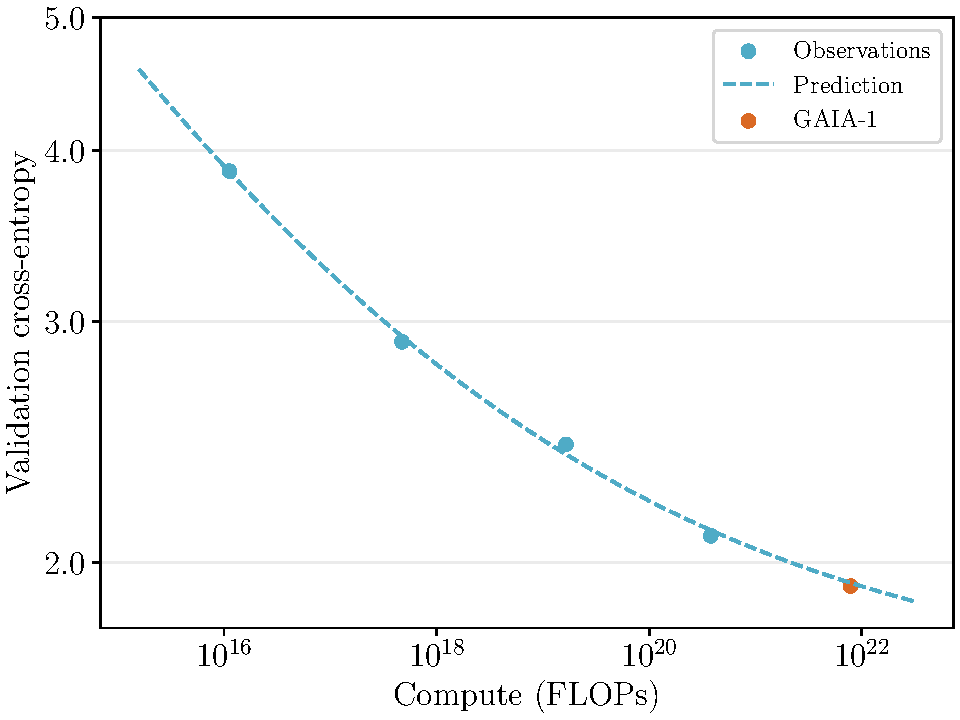
\includegraphics[width=\linewidth]{Figures/Scaling/predict_performance.pdf}%
    \caption{The final performance of the GAIA-1 world model could be predicted with smaller models trained with less than $20\times$ the compute.}
    \label{figure:predict-performance}
    \end{subfigure}\hfill
    %
    \begin{subfigure}[b]{0.49\textwidth}
    \centering
    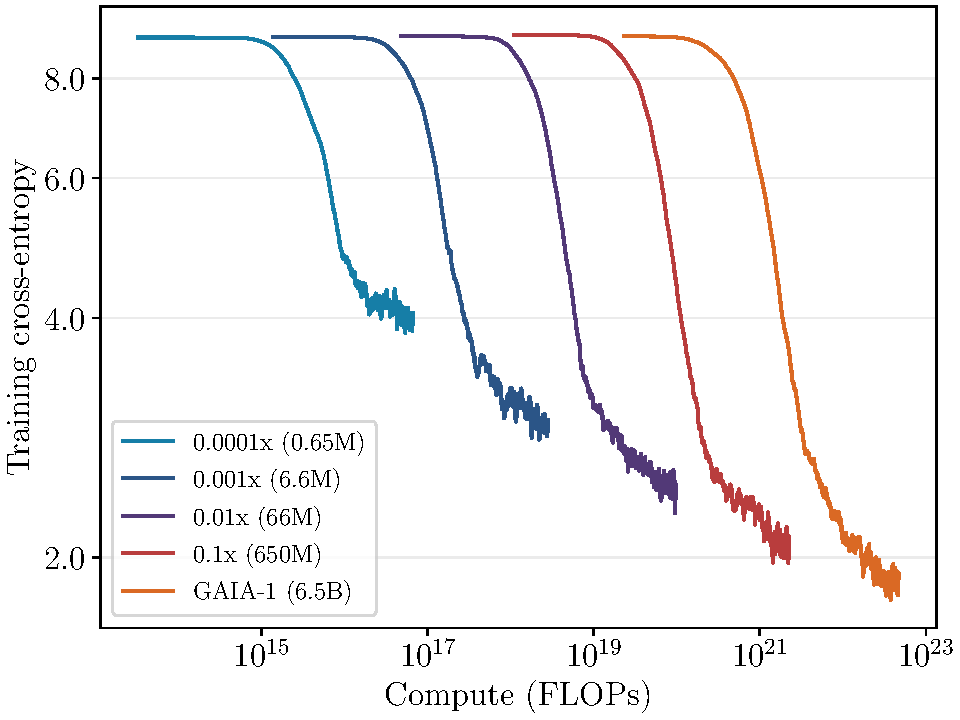
\includegraphics[width=\linewidth]{Figures/Scaling/compute.pdf}%
    \caption{Training loss curves for world models up to 10,000x smaller. We used an exponential moving average to smooth the training loss curves.}
    \label{figure:compute}
    \end{subfigure}
    \caption{Validation and training cross-entropy of the world model.}
\end{figure}

The formulation of the world modeling task in GAIA-1 shares a commonality with the approach frequently used in large language models (LLMs). In both instances, the task is streamlined to focus on predicting the next token. Although this approach is adapted for world modeling in GAIA-1 rather than the traditional language tasks seen in LLMs, it is intriguing to observe that scaling laws \citep{kaplan20, Chowdhery2022PaLMSL,hoffmann22}, analogous to those observed in LLMs, are also applicable to GAIA-1. This suggests the broader applicability of scaling principles in modern AI models across diverse domains, including autonomous driving.

% While scaling enables us to achieve better performance, it does come at the cost of increased inference time: for GAIA-1 it takes 217 seconds to autoregressively generate 576 image tokens with a context of 4880 conditioning and image tokens (corresponding to 8 frames). For the same task, a model with 650M parameters (10 times smaller) takes 36 seconds while a 100 times smaller 66M parameter model takes 10 seconds. These results have been obtained with some out of the box optimizations such as FlashAttention v2 and model compilation at inference time. We do not exclude that further improvements can be achieved.

To explore scaling laws with GAIA-1, we predicted the final performance of the world model using models trained with less than $20\times$ the compute. We evaluated those models on a held-out geofenced validation set by measuring cross-entropy. A power-law of the form $f(x) = c + (x/a)^b$ was then fitted to the data points. In \Cref{figure:predict-performance} we can see that the final cross-entropy of GAIA-1 could be predicted with high accuracy.

The models used to fit the power-law ranged from 10,000x to 10x smaller models in terms of parameters (0.65M to 650M), as visualized in \Cref{figure:compute}. Similarly to \citep{kaplan20}, the compute was estimated as a function of the parameter count. If we denote by $C$ the compute and by $N$ the parameter count (excluding embedding layers), the number of floating point operations for a forward-backward pass of a single token is given by $C=6N$. To obtain the total amount of compute, this value is multiplied by the number of training tokens.



It is worth noting that our extrapolation leads us to the conclusion that there is substantial potential for further improvement through the expansion of both data and computational resources.


